\subsection{Закон Ома в интегральной и дифференциальной формах}

\begin{figure}[h]
    \centering
    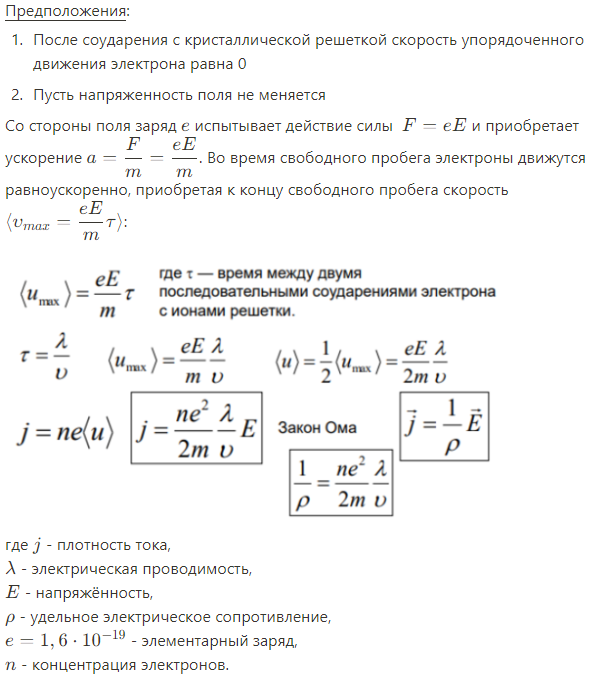
\includegraphics[width = 0.7\linewidth]{imgs/q30i1.png}
\end{figure}

\begin{definition}
    Закон Ома — физический закон, определяющий связь электродвижущей силы источника (или электрического напряжения) с силой тока, 
    протекающего в проводнике, и сопротивлением проводника.
\end{definition}

\begin{definition}
    Закон Ома для неоднородного участка цепи в интегральной форме:

    $$
    I=\frac{(\varphi_1-\varphi_2)+\varepsilon_{12}}{R}
    $$

    При $\varepsilon_{12}=0$ \ \  $I=\frac{\varphi_1-\varphi_2}{R}$ — однородный участок цепи

    При $\varphi_1=\varphi_2$ \ \ $I=\frac{\varepsilon}{R}$ — замкнутая цепь
\end{definition}

\begin{definition}
    В дифференциальной форме при наличии сторонних сил:

    $$
    \vec j=\lambda(\vec E+\vec E_{ст})
    $$

    $$
    \vec j=\frac{\vec E}{\rho}=\lambda\vec E
    $$

    Связывает плотность тока $j$ в любой точке внутри проводника с напряженностью $E$ электрического поля в этой же точке.
\end{definition}